\documentclass[10pt,a5paper,twoside]{book}
\usepackage[utf8]{inputenc}
\usepackage[czech]{babel}
\usepackage[T1]{fontenc}
\usepackage{amsmath}
\usepackage{amsfonts}
\usepackage{amssymb}
\usepackage{hyperref}
\usepackage[dvips]{graphicx}
\usepackage[top=2cm, left=1.5cm, bottom=1.5cm, includefoot]{geometry}
\usepackage{eso-pic}
\usepackage{pdfpages}
\usepackage{textpos}
\usepackage{titlesec}
\usepackage{verbatim}
\fontencoding{T1}
\fontfamily{cmss}
\fontseries{m}
\fontshape{n}
\setlength{\belowcaptionskip}{-15pt} % mezera za popiskem obrázku
\usepackage{xcolor}
\usepackage{pdfpages}
\titleformat{\section}
{\color{blue}\normalfont\Large\bfseries}
{\color{blue}\thesection}{1.2em}{}

\newcommand{\autor}[1]{
	\begin{flushright}
	\textit{#1}
	\end{flushright}
}

\newcommand{\nadpis}[2]{
\section*{#1}
	\begin{flushright}
	\textit{#2}
	\end{flushright}
}

\newcommand{\podpis}[1]{
	\begin{flushright}
	\textit{#1}
	\end{flushright}
}

\begin{document} 



\section*{K obrázku na titulní straně}
Venčení Psa a páníčka Astronoma při pozorování Galileovských měsíců po tom, co se zatáhlo nad jižním obzorem při hledání komety C/2014 Q2 \hbox{(Lovejoy)} z kopce poblíž obce Strážkovice. Kometa byla po nějaké době krátce zahlédnuta v triedru do doby, než se znovu zatáhlo.
\autor{Roman Dvořák}
\vfill
\section*{JihoČAS}
Vydává: Jihočeská pobočka České astronomické společnosti.\\
Redakce a adresa pro zasílání příspěvků: Martin Kákona, U Jatek 19/III, 392 01 Soběslav, e-mail: \href{mailto:martin.kakona@astro.cz}{martin.kakona@astro.cz}.\\
Sazba: Roman Dvořák, e-mail: \href{mailto:roman-dvorak@email.cz}{roman-dvorak@email.cz}.\newpage

\nadpis{Členská schůze}{}
Letošní členská schůze proběhla netradičně ve Svákovské hvězdárně v Soběslavi. Důvodem byla právě probíhající rekonstrukce Hvězdárny Fr. Pešty, takže jsme se sešli mimo pořadí na novém místě.

\begin{figure}[htbp]
	\begin{center}
		\includegraphics[width=7cm]{schuze/sch_02.eps}
	  	\caption{Hvězdárna a meteorická observatoř Svákov – Soběslav, aneb, jak se stoupá ke hvězdám.}
	  	\label{fig:}
	\end{center}
\end{figure}
\par
Schůze se zúčastnilo 11 astronomů a astronomek. Jednalo se nejen o duchovní ale také o kulinářský zážitek. Kromě již tradiční rolády z Prahee jmenujme z dalších dobrot například piškot s báječnou smetanovou chutí nebo sýrovou pomazánku s hebkou plísní. Jídla byl skutečně dostatek, takže děti z kroužku, který se ještě týž den sešel ve večerních hodinách, měli výtečnou večeři.

Duševní potravou pak byly tyto přednášky:
\begin{itemize}
\item Stav sítě Bolidozor \textit{(Martin Kákona)}
\item Datamining ze space.astro.cz \textit{(Josef Szylar)}
\item Autonomní robotické observatoře \textit{(Jan Štrobl)}
\end{itemize}

Shlédli jsme také některé interesantní historické dokumenty z dávných dob Hvězdárny Fr. Nušla.
Při prohlídce Svákovské hvězdárny hosté věnovali zvláštní pozornost biologickým sekačkám trávy v okolí anténního systému pro KV pozorování.

Lze shrnout, že se jednalo o příjemně strávený den v kruhu podobně smýšlejících lidí.

\begin{figure}[htbp]
	\begin{center}
		\includegraphics[width=9cm]{schuze/sch_03.eps}
	  	\caption{Kolargon z hvězdárny v J.Hradci na plošině s demonstrátorem u ufiště reflektoru.}
	  	\label{fig:}
	\end{center}
\end{figure}

\begin{figure}[htbp]
	\begin{center}
		\includegraphics[width=9cm]{schuze/sch_04.eps}
	  	\caption{Vedoucí observatoře a Sanny Trostová ze Sezimova Ústí před schůzí ČASu.}
	  	\label{fig:}
	\end{center}
\end{figure}

\begin{figure}[htbp]
	\begin{center}
		\includegraphics[width=9cm]{schuze/sch_05.eps}
	  	\caption{Antény.}
	  	\label{fig:}
	\end{center}
\end{figure}

\nadpis{O hřevulích s ohnivým ohonem\\\textit{Několik poznámek k vývoji české terminologie}}{Alena Šolcová}
\begin{flushright}
\textit{Velmi potěšitelné jest, že v naší milé vlasti \\
všecky téměř vědy nalézají učených pěstitelů, \\
jenž je  v rauše mateřské řeči \\
vzdělanému obecenstvu podávají …}
\end{flushright}

V poslední době mě zaujal vývoj české odborné terminologie. Velmi zajímavé jsou spisy z první poloviny 19. století. V díle nazvaném \textbf{Nebe a země klíč, čili:  \textit{všesrozumitelní začátkové učení o nebi a zemi}} od Antonína Vojtěcha Hnojka z roku 1843  (viz [2]) najdeme ukázky toho, jak byl vývoj odborné češtiny složitý a znalosti o objektech ve vesmíru jiné.
\par
Rozsáhlé dílo zahajuje autor výkladem o nebeské obloze, o obzoru a hvězdnatém nebi a čtenářům ve 30 kapitolách vysvětluje pojmy užívané v~\hbox{astronomii} a příbuzných oborech. Ve 13.  kapitole popisuje planety, \hbox{sputníky} a hřevule (viz [2], str. 34-37). 
\par
Pro planety užívá další slova – \textbf{oběžnice, družice, bludice, pobludice} a přidává ještě tehdy obvyklé německé termíny – \textit{die Planeten, Irrsterne, Wandelsterne.}
\par
Čtenářům předkládáme hádanku, jaké planety, trpasličí planety a planetky se skrývají za poetickými názvy: \textbf{Dobropán, Krasopaní, Tellus,  Smrtonoš, Čistěna, Královna} aneb \textbf{Jovina, Živěna, Mudřena, Kralomoc, Hladolet, Nebešťanka}. Rozluštění najdete na konci článku.  V té době se podle autora točilo okolo Slunce 11 planet.  Další tělesa jsou zvána také hvězdy:
\par
\textit{„A okolo několika těch planet točí se také hvězdy, kteréž slovau jejich sputníci, družice, trabanti (ihre Nebenplaneten, Trabanten) …“} (viz [2], str. 34).
\par   
Pak vysvětluje tajemné slovo  \textbf{\textit{„hřevule“}}.  Jsou to tělesa obyčejně vlekoucí za sebou dlouhý, světlý, jako ohnivý ohon, podobný vlasům či hřívě, takže je nazývá také \textbf{\textit{ohonice}} (die Schwanzsterne), \textbf{\textit{vlasatice}} (die Haarsterne). Upozorňuje, že odtud je také převzato jméno \textit{\textbf{kometa}}, které je řeckého původu a znamenalo původně vlasy na hlavě neboli kštici.
\par
U českých pojmů autor uvádí jejich německé ekvivalenty. Uvědomme si, že zatímco v němčině byla již odborná terminologie rozvinuta, v češtině tehdy vědci teprve hledali nové  termíny. Jen některé z nich se však ujaly. V textu najdeme např. výraz pro zvěrokruh: \textbf{zvířetník}, ale též \textbf{zemokrut (der Thierkreis, Zodiacus)}. Ekliptiku autor zkouší nazvat \textbf{slunečníkem} i \textbf{slunníkem}. Pro některé pojmy ještě označení není a používá se opis, např. \textbf{„letní zastavení se“}, čili \textbf{„letní obrat slunce“} pro slunovrat. 
\par
Volba názvu pro kometu – hřevule – je vhodná. Autor sám si pochvaluje:
\par
\textit{„Dobřeť se nazývají hřevule, poněvadž bývá ten rok neobyčejně teplý, kdy se kometa na nebi okáže. Takový rok byl 1811, kdežto bylo viděti kometu s ohonem 22 miliónů mil dlauhým. Toho roku výborné \textbf{víno} slaulo \textbf{kometové},“}  (viz [2], str. 36).   
\par
Poznatky o kometách ze čtyřicátých let 19. století nás mohou dnes překvapovat: Hřevule vznikají ze slunečních výparů, dosud nejsou dosti pevné, jsou nedozrálé, teprve časem se mají stát oběžnicemi a obydlím živých tvorů jako je naše Země. Jejich hmota je řídká a tak průhledná, že skrz okraj jejich jádra je vidět i ty nejmenší hvězdy v neoslabeném lesku. Je třeba, aby ztuhly a zpevněly. A autor si zavzpomíná: \textit{„Snad naše Země také někdy – ale Bůh sám ví, jak dlauho tomu jest – byla kometau.“}  Pak  popisuje, že komety mají s ohonem svým podobu metly nebo ohnivého meče. Některé hřevule jsou bez ohonu a \textit{„vyjevují se jen co pauhé kotauče parné těla neurčitého.“} 
\par
Vzpomíná také Halleyovu kometu, která se ukázala v říjnu 1835.  \textit{„Mimo tuto vlasatici znají hvězdoslovci ještě tři, jejichž čas oběžní vypočítán jest. Tak zvaná Olbersova od roku 1815, okáže se teprve roku 1890.“} Upozorňuje také, v letopisech jsou zprávy o 400 kometách, ale jen 121 bylo „hvězdoskumně“ pozorováno. 
\par
Nakonec utěšuje čtenáře, že \textit{„ačkoliv komety dokonce jinák nežli jiné hvězdy běží, nicméně hvězdářové umějí vypočítati, za kolik let se některé aspoň naším očím opět na obloze okáží. Vesměs, prý, vracejí se tytéž komety asi za 500 roků, aby od nás vidíny byly,“} (viz [2], str. 35).       
\par 
Dnes máme o kometách docela jiné znalosti. V přehledném a srozumitelném výkladu o fyzice Sluneční soustavy (viz [1]) si připomeneme, že komety – hřevule jsou obvykle tělesa tvořená směsí prachu a ledu, který se při přiblížení ke Slunci přeměňuje na plyn a spolu s prachem pak uniká z gravitačního pole komety. Obvykle mívá kometa dva ohony, jeden iontový - namodralý (směřuje radiálně od Slunce) a zakřivený prachový - nažloutlý. Mikroskopické prachové částice jsou ovlivněny tlakem záření Slunce, a proto se pohybují po jiných trajektoriích než jádro komety. Pozoruhodný je také vývoj pojmenování komet – hřevulí. Před rokem 1900 se komety jmenovaly jednoduše „Velká kometa roku …“ (1557, 1680), nebo např. Velká lednová kometa 1910, jasnější než Halleyova, pozorovatelná v květnu téhož roku. Jinak se komety jmenují také po lidech, kteří zkoumali jejich dráhy, např. Halley, Encke, Biela.  V letech 1900 až 1964 se používalo označení: rok objevu, písmeno pořadí objevu (např. 1976 n = kometa West, 1983 i = Halleyova kometa). Definitivní označení se stanovuje podle roku a pořadí průletu periheliem (1986 III = 1983 i = Halleyova kometa). Od roku 1994 se používá předběžného označení ve tvaru C/1995 O1 (Hale-Bopp), kde O je polovina měsíce, 1 je pořadí objevu a v závorce je jméno pozorovatele nebo max. dvou pozorovatelů. Písmena před lomítkem mohou být C = neperiodická kometa, P = periodická kometa, X = kometa pozorovaná jen jednou, D = zmizelá kometa a A = omyl (např. asi planetka).  Poutavý výklad o proměnlivé aktivitě komet – hřevulí a o jejich skladbě najdete v [1]. \\  \\
\textbf{Poznámka:}\\ Citáty jsou pro lepší čitelnost uvedeny v transliterované podobě \\
g -> j,  w -> v, j -> í. \\ \\ \\ \\  \\
\textbf{Použitá literatura:}\\
{[}1{]} Brož, M., Šolc, M.: Fyzika sluneční soustavy. Matfyzpress, MFF UK Praha, 2013.\\
{[}2{]} Hnogek, A. V.: Nebe a země kljč, čili: wšesrozumitelnj začátkowé učenj o nebi a zemi. Tiskem Anny ovdowělé Špinkowé, W Praze 1843.\\ \\
\textbf{Rozluštění:\\Dobropán} = Merkur,  \textbf{Krasopaní} = Venuše, \textbf{Smrtonoš} = Mars, \textbf{Čistěna} = Vesta, \textbf{Královna} nebo \textbf{Jovina}  =  Juno, \textbf{Živěna} = Ceres, \textbf{Mudřena} = Pallas, \textbf{Kralomoc} = Jupiter, \textbf{Hladolet} = Saturn, \textbf{Nebešťanka} = \textbf{Uran} a \textbf{Země} je Tellus.

\nadpis{Doplňující údaj ke kresbě kráteru Clavius}{Milan Blažek,\\ Hvězdárna a planetárium hl. m. Prahy, p. o.}

Vážení čtenáři JihoČASu. Kresbu kráteru Clavius (stínovanou fixem) jste možná někteří již mohli spatřit jinde. Rád bych zde uvedl na pravou míru neúplný popisek, který se u ní bohužel (hlavně vinou nedostatku místa a časové tísně autora i vydavatele) vyskytl. Uvádí se v něm, že se jedná o kresbu z pozorování - viz. tento popisek:  \\

\textbf{\\
Datum pozorování: 24. března 2010\\
Místo pozorování: Štefánikova hvězdárna, Praha - Petřín\\
Čas pozorování: 21.52–23.04 UT\\
Colongitudo: $23,9 ^\circ$\\
Název útvaru: Clavius\\
Autor kresby: Milan Blažek (HaP Praha, p. o.)\\
Pořadové číslo: $501$\\
Dalekohled: meniskus Cassegrain 350/3300 mm\\
Zvětšení: $206 \times $ \\
Kvalita obrazu: dobrá \\
Přesnost zákresu: velmi dobrá\\}

\newpage
\begin{figure}[htbp]
	\begin{center}
		
\includegraphics[width=12cm]{blazek/0501.eps}
	\end{center}
\end{figure}

Ano, v tomto termínu jsem skutečně zmiňovaný útvar pozoroval, ale již na první pohled je patrné, že tak složitou oblast bych takto detailně za zmiňovaný časový úsek u dalekohledu nestihl zakreslit (ani jako tzv. pérovku).

Jedná se v podstatě o překreslenou fotografii, kterou nasnímal (15. února 2008 v 18 h 58 min UT) a následně počítačově zpracoval pan François Emond, od něhož jsem si vyžádal svolení k překreslení. Kresbu uveřejňuji s laskavým souhlasem autora snímku. Z mého pozorování jsou do kresby zakomponovány pouze částečné změny v rozložení ploch stínů. 

Jak vypadá kresba z (jiného) přímého pozorování dalekohledem, v tomto případě bez pomoci fotografie, se můžete podívat na zákresu pořízeném tužkou.  \\
\newpage
\textbf{\\Datum pozorování: 4. dubna 2009\\
Místo pozorování: Štefánikova hvězdárna, Praha - Petřín \\
Čas pozorování: 21.02 – 21.43 UT\\
Colongitudo: $27,8 ^\circ$\\
Název útvaru: Clavius\\
Autor kresby: Milan Blažek (HaP Praha, p. o.)\\
Pořadové číslo: $410$\\
Dalekohled: meniskus Cassegrain 350/3300 mm\\
Zvětšení: $132\times$ \\
Kvalita obrazu: velmi dobrá až dobrá \\
Přesnost zákresu: velmi dobrá\\}

\begin{figure}[htbp]
	\begin{center}
		\includegraphics[width=12cm]{blazek/0410.eps}
	\end{center}
\end{figure}
\newpage

\nadpis{Hustý!}{Martin Kákona}
Nedávno jsem si všiml ve slovníku mojí dcery tohoto zajímavého slova. Jedná se zřejmě o moderní výraz pro téměř vše, co stojí v našem Vesmíru za pozornost. Pojďme se tedy společně podívat na to, jak je náš Vesmír vlastně hustý.
\par
Začneme pěkně po pořádku od toho nejmenšího co známe, k tomu největšímu kam dohlédneme. 
\par
Takže nejdříve kvarky a elektrony. (Trochu si to zjednodušíme, nebudeme hovořit o mionech, tauonech a podobných nestabilních částicích a také zanedbáme dosud neobjevené částice a jejich antičástice ;) Kvarky a elektrony se nacházejí v atomech. Přičemž kvarky pro sebe potřebují prostor přibližně $10^{-15}$ m a elektrony $10^{-10}$ m. Kvarků je v atomu většinou 6x více než elektronů a zabírají 100000x menší prostor. Dá se tedy říci, že jádro atomu je husté a atom je naproti tomu řídký. Nicméně, z pohledu dalších částic, které zde zmíníme, neutrin, je celý atom velmi řídký. Pokud vezmeme něco většího, co je poskládáno z atomů, třeba vás, tak po dobu, co čtete tento článek, vámi prolétne přibližně 1015 neutrin (což je rozpočet naší republiky na 1000 let v korunách za předpokladu stejné hodnoty koruny po celou dobu). Když budete mít štěstí, tak se do vás, než tento článek dočtete, i jedno neutrino trefí a než umřete možná i druhé. Takže člověk zrovna moc hustý není.
\par
Vezměme tedy něco většího. Třeba Slunce. Slunce je v průměru jen o něco málo hustší než člověk. Ovšem důležité je to „v průměru“. Zatímco v centru je Slunce 1000x hustší než my (tedy z pohledu neutrin furt nic moc), tak na povrchu (pokud se dá o povrchu hovořit), je Slunce řidší než atmosféra na Zemi. Pokud budeme za povrch Slunce považovat to, co z něj běžně vidíme, tady fotosféru, tak zde hustota odpovídá naší atmosféře ve výšce cca 60km. 
Dále od Slunce průměrná hustota vesmíru stále klesá. Ve vzdálenosti od Slunce, ve které právě sedíte, se v každém $cm^{3}$ Vesmíru nachází pouze desítky kvarků i když bezprostředně kolem vaší židle je lokálně hustota mnohem větší a nikam se nepropadnete. Takových lokálních zhustků hmoty je ve vesmíru mnoho a některé jsou velmi velmi husté. Nicméně, průměrná hustota galaxií a ještě větších útvarů je velmi velmi malá. 
\par
Takže prostor mezi hvězdami je řídký. Je dokonce tak řídký, že atomy plynů v něm nejsou spořádaně ve dvojicích, jako je tomu v atmosféře Země, ale jsou v tomto řídkém prostoru po jednom. Přesto je ale mezi hvězdami něco, čeho je celkem hodně, co nevidíme, ale jako hmota se to chová a je to vlastně z pohledu viditelné hmoty velmi husté, protože je toho 25x víc.
\par
A co prostor za naší galaxií? Tedy mezigalaktický prostor? No tak ten je tedy ale opravdu řídký! Kdybyste z naší galaxie vylétli do prostoru mezi galaxiemi, bylo by to, jako kdybyste z vody vylétli do vzduchu. Celkem by mne zajímalo, jestli pro tento případ také platí Archimédův zákon. Víme totiž, že s tímto velmi řídkým prostorem je něco v nepořádku. Víme, že v tom ničem něco je, a že se to snaží viditelnou i neviditelnou hmotu stále ředit. Takže pokud je náš vesmír z našeho pohledu dnes řídký, bude jednou ještě řidší.
\par
Vidíme tedy, že náš Vesmír je vlastně řídký a stále se zřeďuje. Na druhou stranu to, co nevidíme, toho je vlastně ve Vesmíru nejvíc. A Tak si myslím, že je ten náš Vesmír vlastně „hustý“ a stojí za to, ho pozorovat.
\begin{figure}[htbp]
	\begin{center}
		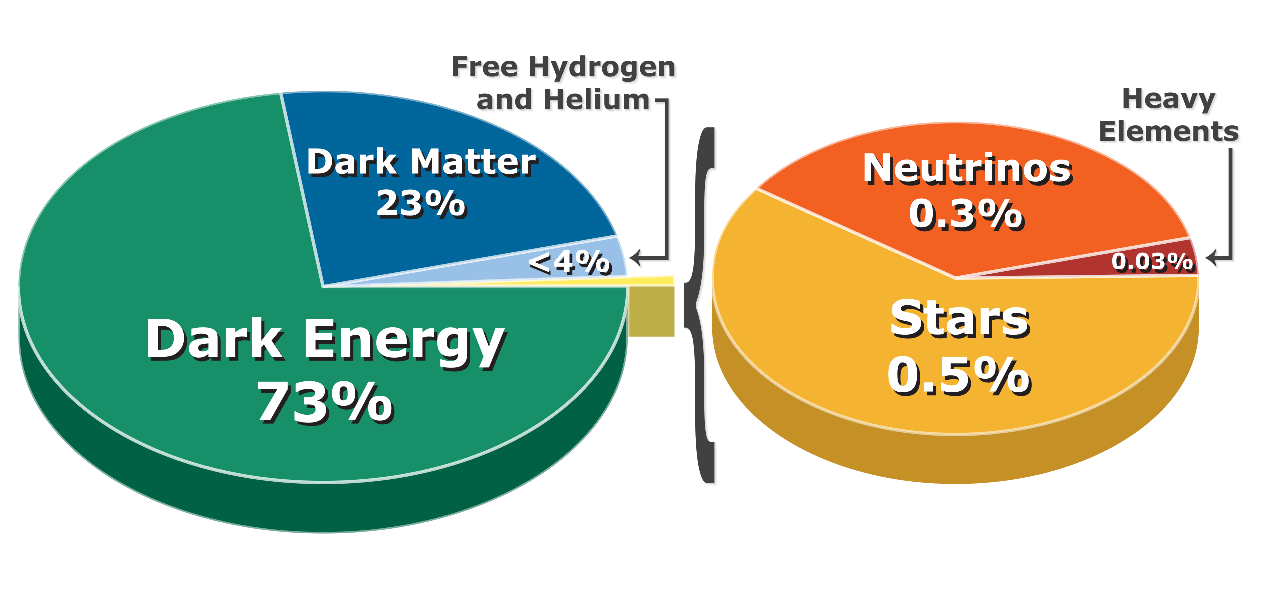
\includegraphics[width=12cm]{husty.eps}
	  	\caption{Rozložení hmoty/energie ve Vesmíru. Hodnoty jsou pouze přibližné a stále se mění současně s novými poznatky.}
	  	\label{fig:}
	\end{center}
\end{figure}
%\newpage
%\section*{Vyhledávací mapa komety C2014/Q2 (LOVEJOY)}
%\begin{figure}[htbp]
%	\begin{center}
%		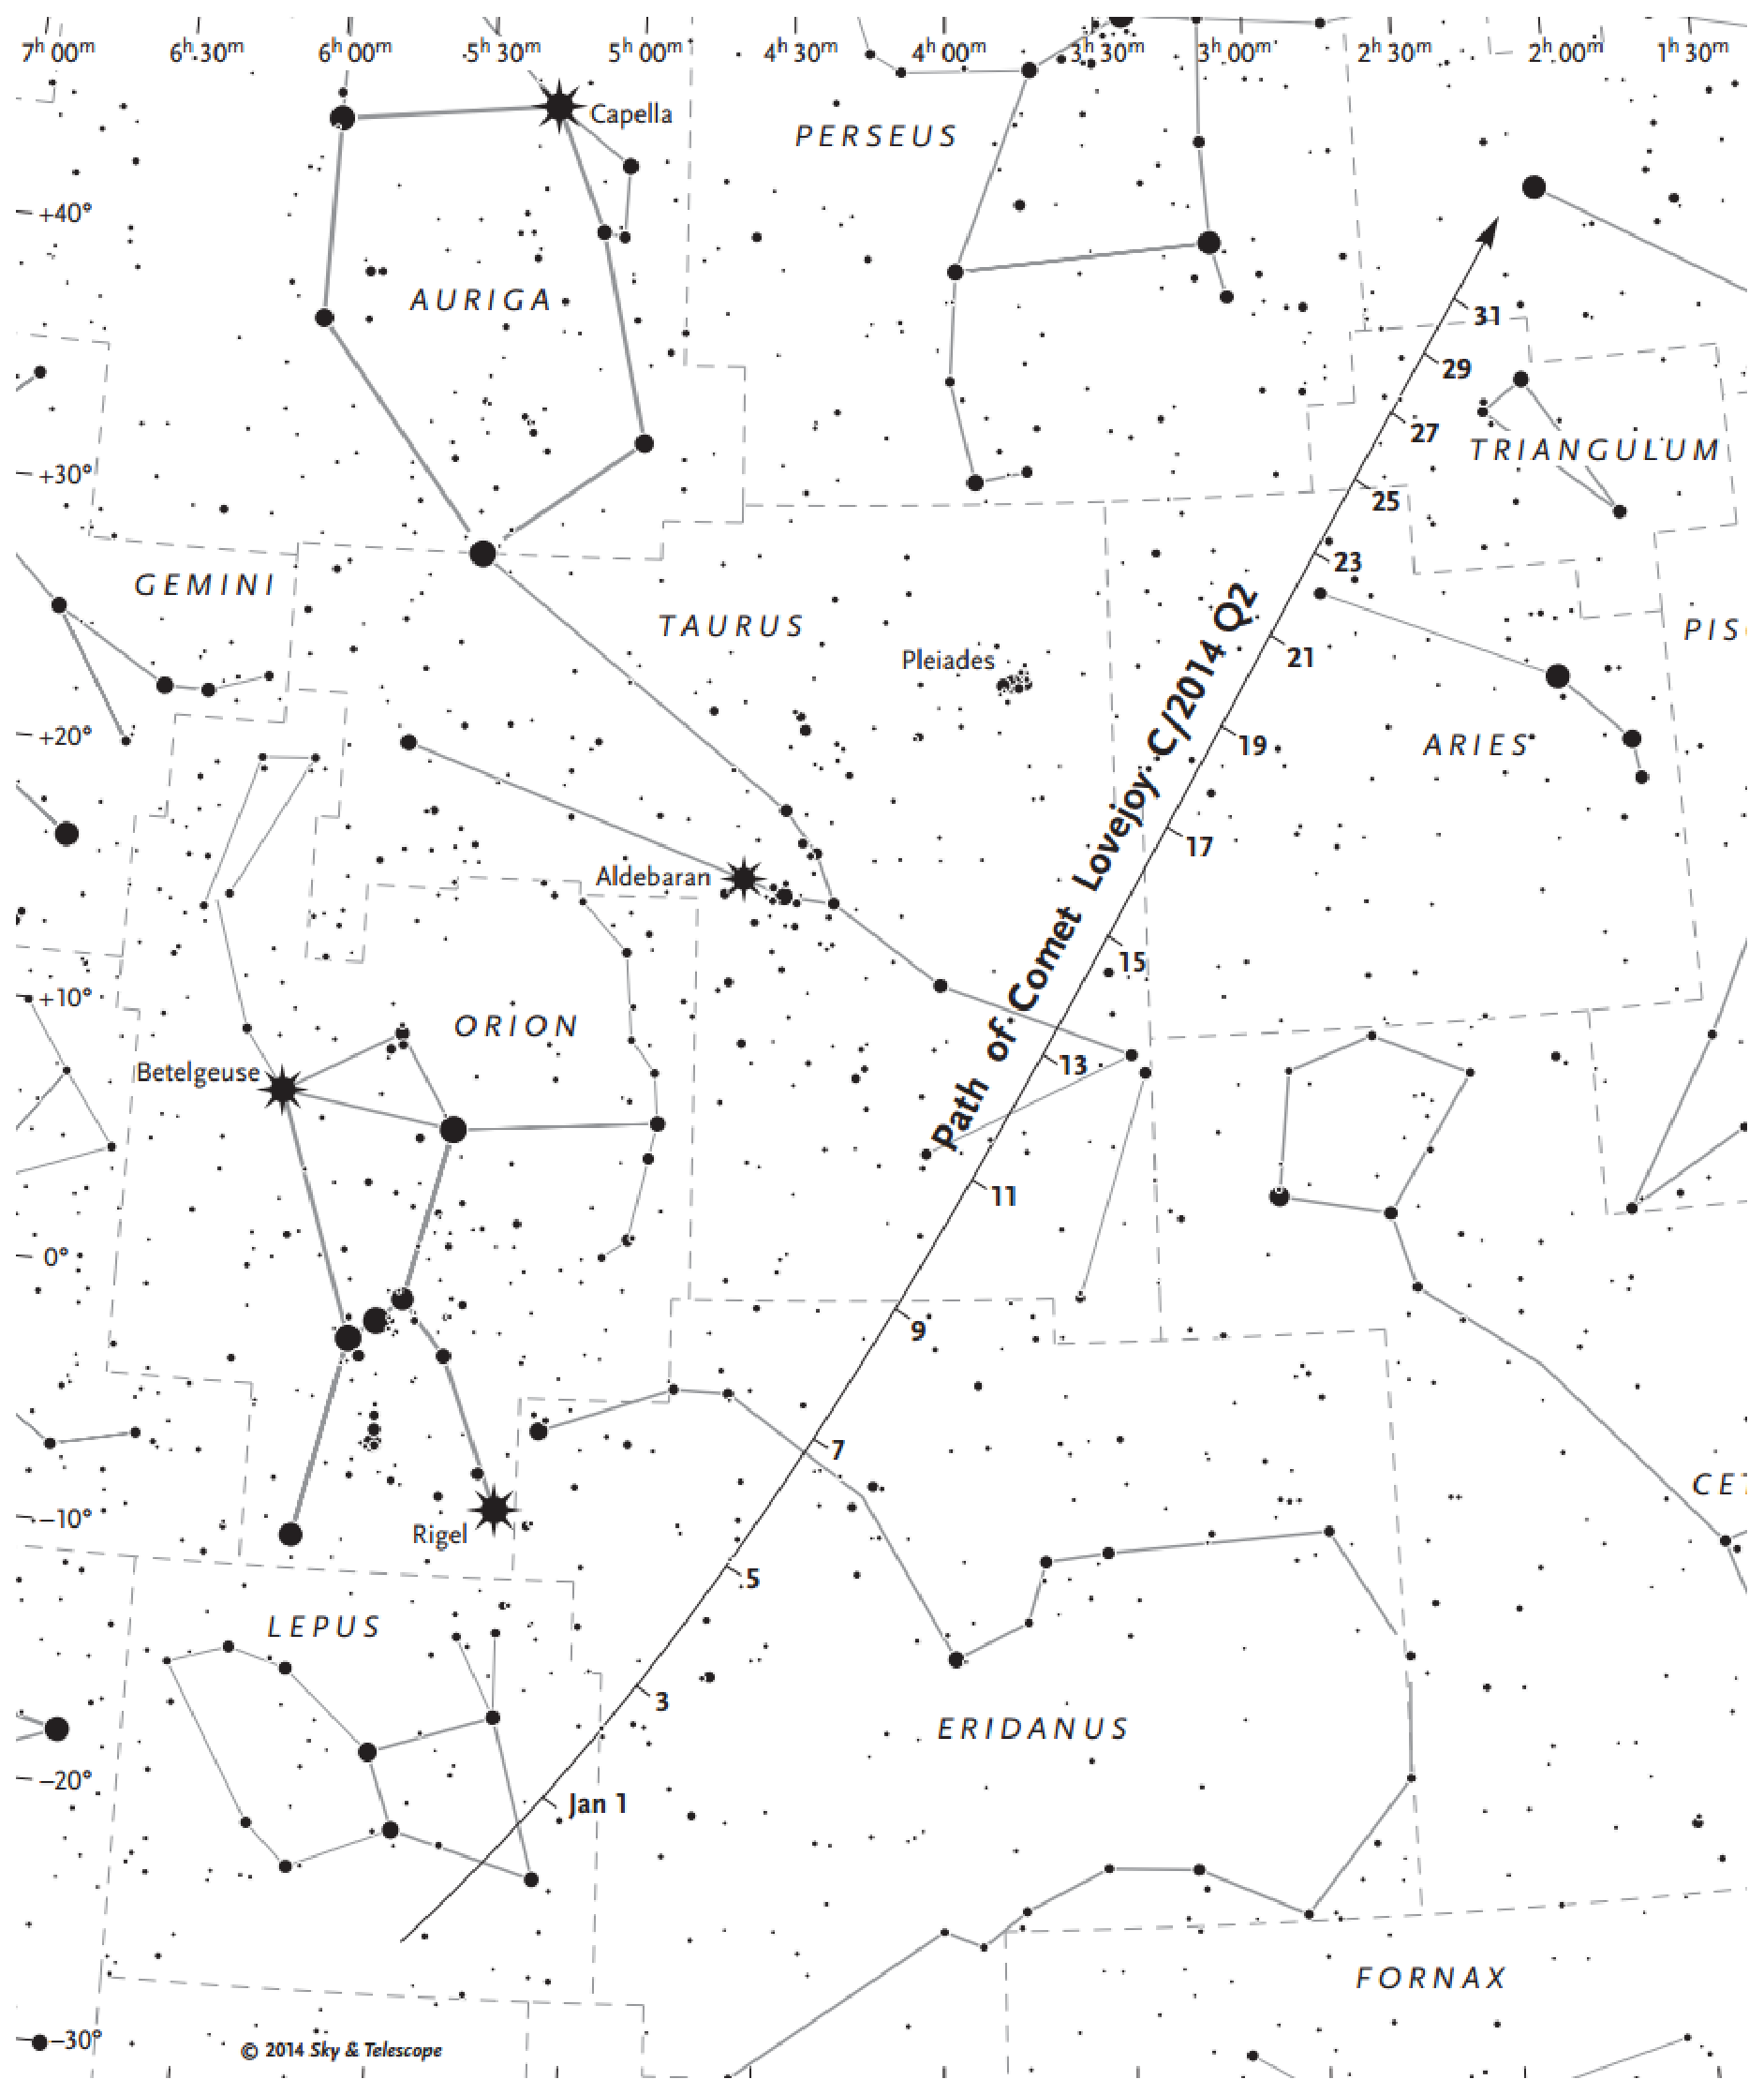
\includegraphics[width=10cm]{c2014q2.eps}
%	\end{center}
%\end{figure}
\end{document}
 
 
%	\begin{itemize}
%	\item 
%	\end{itemize}
